
\documentclass{sice-si}
% タイトルと著者名
\title{視覚と行動のend-to-end学習により経路追従行動を\\
オンラインで模倣する手法の提案\\
トポロジカルマップとシナリオに基づく経路選択機能の追加と検討\\
}
\name{○春山 健太(千葉工大),藤原 柾(千葉工大)} % 著者名
\etitle{Instruction for SICE SI Annual Conference Manuscript} % 英文タイトル
\ename{○Kenta HARUYAMA (CIT), and Masaki Fujiwara (CIT)}	%著者名(英)

\begin{document}
% アブストラクト
\abst{
    This manuscript describes a method for preparing a manuscript for the annual conference of the SICE SI division.
}

% タイトルの出力
\maketitle

% 本文
\section{緒言}
本研究グループでは,end-to-end 学習により,カメラ画像を
入力として,経路を追従する行動をオンラインで模倣する手
法を提案している.[春山]では,これに経路を選択する機能を追加し,
[藤原]では成功率の不均衡データの緩和,
積極的な蛇行により学習時間の短縮を行っている.
この手法(以後,本手法と呼ぶ)をシミュレータや実ロボットを用いた
実験により有効性を検証した.本手法は,地図に基づく経路追従行動を模
倣して,〜のようなカメラ画像を入力とする経路追従行動
を生成する.さらに,分岐路などで目標とする進行方向(以後,目標方向
と呼ぶ)に応じて,経路を選択して走行する.本手法により,
地図に基づく経路追従とカメラ画像を入力とする経路追従の
2 つのナビゲーション手段が得られる.この 2 つの手段を状況
に応じて高い信頼性が見込まれる方を選択することで,
経路追従を継続できる可能性が高まる.
[春山]や[藤原]では,訓練後の学習器を用いた走行に用いる目標方向の生成を
地図に基づいた制御器を用いて行っていた.
カメラ画像を用いて目的地へ到達するためには,
カメラ画像のみに基づいて目標方向を生成する必要性がある
本稿では,[春山]や[藤原]で行ってきた経路選択機能を追加した手法へ,
カメラ画像を用いた目標方向の生成方法の追加目的として
トポロジカルなプランナの追加を行う.
これにより地図に地図に基づいた制御器への依存をなくし,
カメラ画像のみに基づいて指定された経路に沿って走行し,
目的地へ到達することが期待される.
本稿では,〜に対して目標方向の生成,経路の指示を行うナビゲーションの追加について議論する.
また,実ロボットを用いた実験を通して,有効性を確認する.


\section{提案手法}
\subsection{目標方向によって条件付けた模倣学習}
基本的な流れ
オーバーサンプリング
積極的な蛇行
\begin{figure}[htbp]
    \begin{center}
    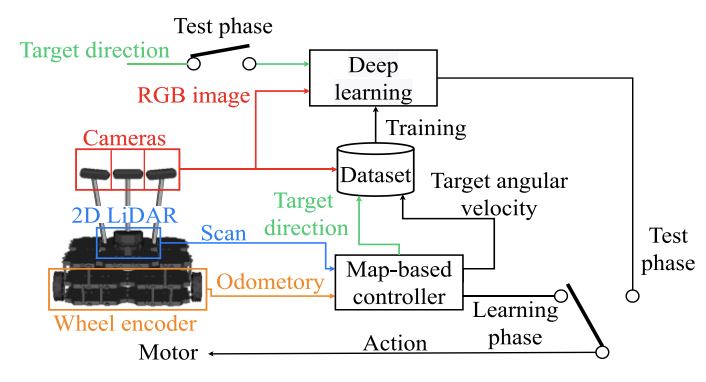
\includegraphics[width=70mm,height=50mm]{./figs/imitation.png}
    \caption{imitation}
    \end{center}
    \label{fig:imitation}
\end{figure}

\subsection{目標方向を生成する〜}
\subsubsection{シナリオ}
目的地までの経路の設定及び,目標方向の生成を行う通路の特徴に基づいた
ナビゲーション手法について述べる
この手法は島田らがアンケートから得た,人が道案
内利用する,向いている方向や突き当たりなどの通路情報
に関する情報を含有した,ナビゲーションに用いるトポ
ロジカルマップとシナリオ(経路の表現)の形式を提案し,実ロ
ボットを用いた実験により提案したナビゲーション手法の有効性
を検証している.
島田らは1.シナリオからロボットの制御用の手順を生成する機能,2.通路の特徴を検出する機能
3.経路に沿って通路を走行する3つの機能を開発している.
本稿では1.のシナリオからロボットの制御用の手順を生成する機能のみを用いる.


\subsubsection{カメラ画像を用いた通路分類}
カメラ画像に基づいた通路分類器について述べる.
通路分類器の概要を〜に示す.通路分類器は
一連のカメラ画像を入力とし,現在の通路の特徴の分類を出力する.
これによりLiDARや全天球カメラ
分類する通路の特徴は島田らに倣い,\ref{fig:intersection}に示した8つに分類する.
\begin{figure}[htbp]
    \begin{center}
    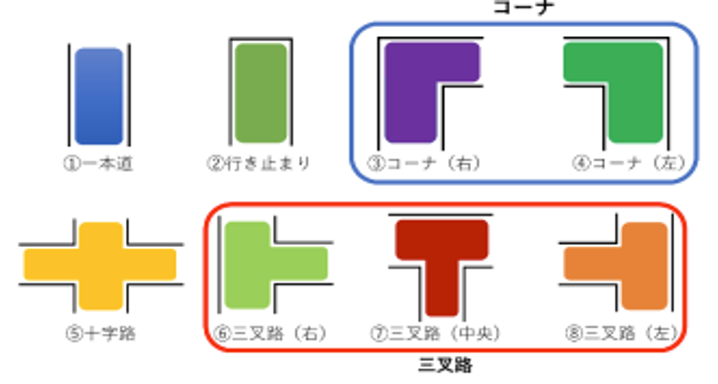
\includegraphics[width=70mm,height=50mm]{./figs/intersection.png}
    \caption{intersection}
    \end{center}
    \label{fig:intersection}
\end{figure}
具体的なネットワーク構造を図〜に示す.構造に関してD.バットらが提案したCNNとLSTMを組み合わせた
LRCNをアーキテクチャを参考としている.
フレーム数は16 入力画像サイズは64✖️48 出力8としている.
\begin{figure}[htbp]
    \begin{center}
    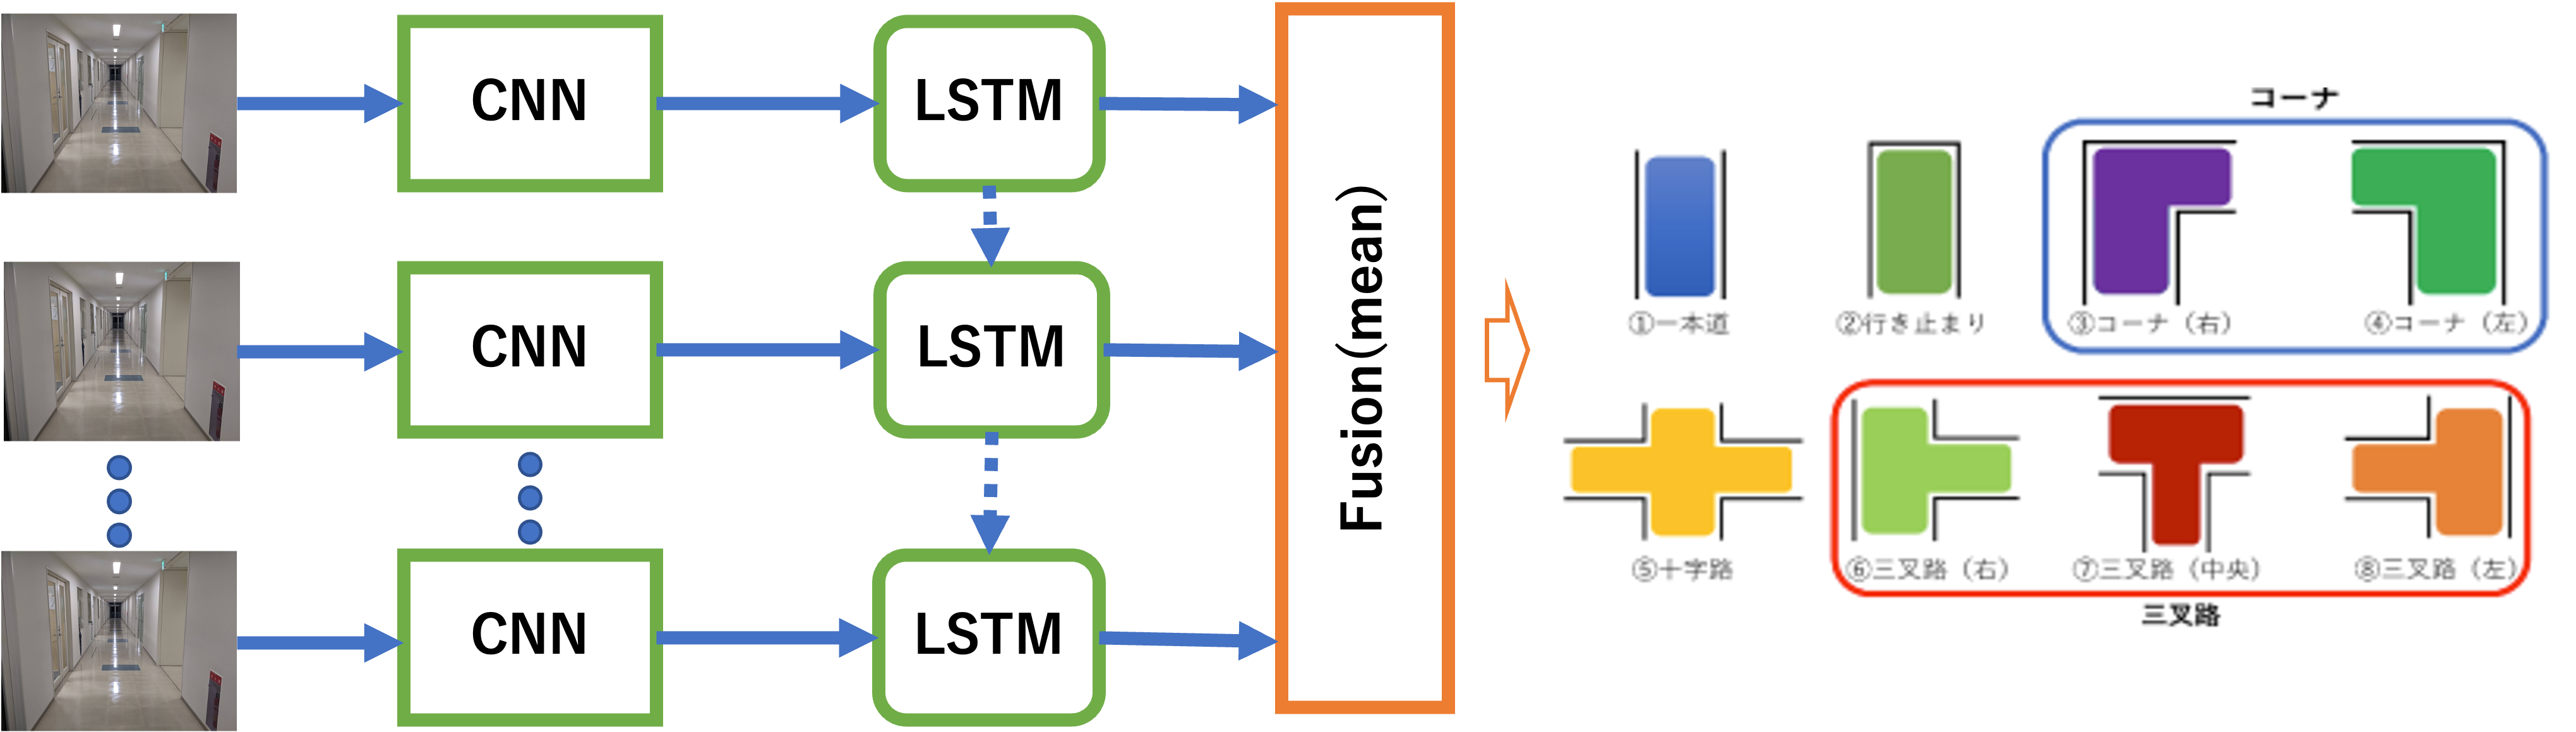
\includegraphics[width=70mm,height=30mm]{./figs/LRCN.png}
    \caption{LRCN}
    \end{center}
    \label{fig:LRCN}
\end{figure}
通路の分類の範囲の図の話
通路の検出タイミングの話

\section{実験}
カメラ画像を入力とする学習器へ島田のナビゲーションを加えた
システムを組み合わせた実験を行います.
\subsection{実験装置}
実験装置を〜に,またセンサ構成を〜に示す.
本学で開発しているorne gammaをベースにカメラを3つ追加している.

\begin{figure}[htbp]
    \begin{center}
    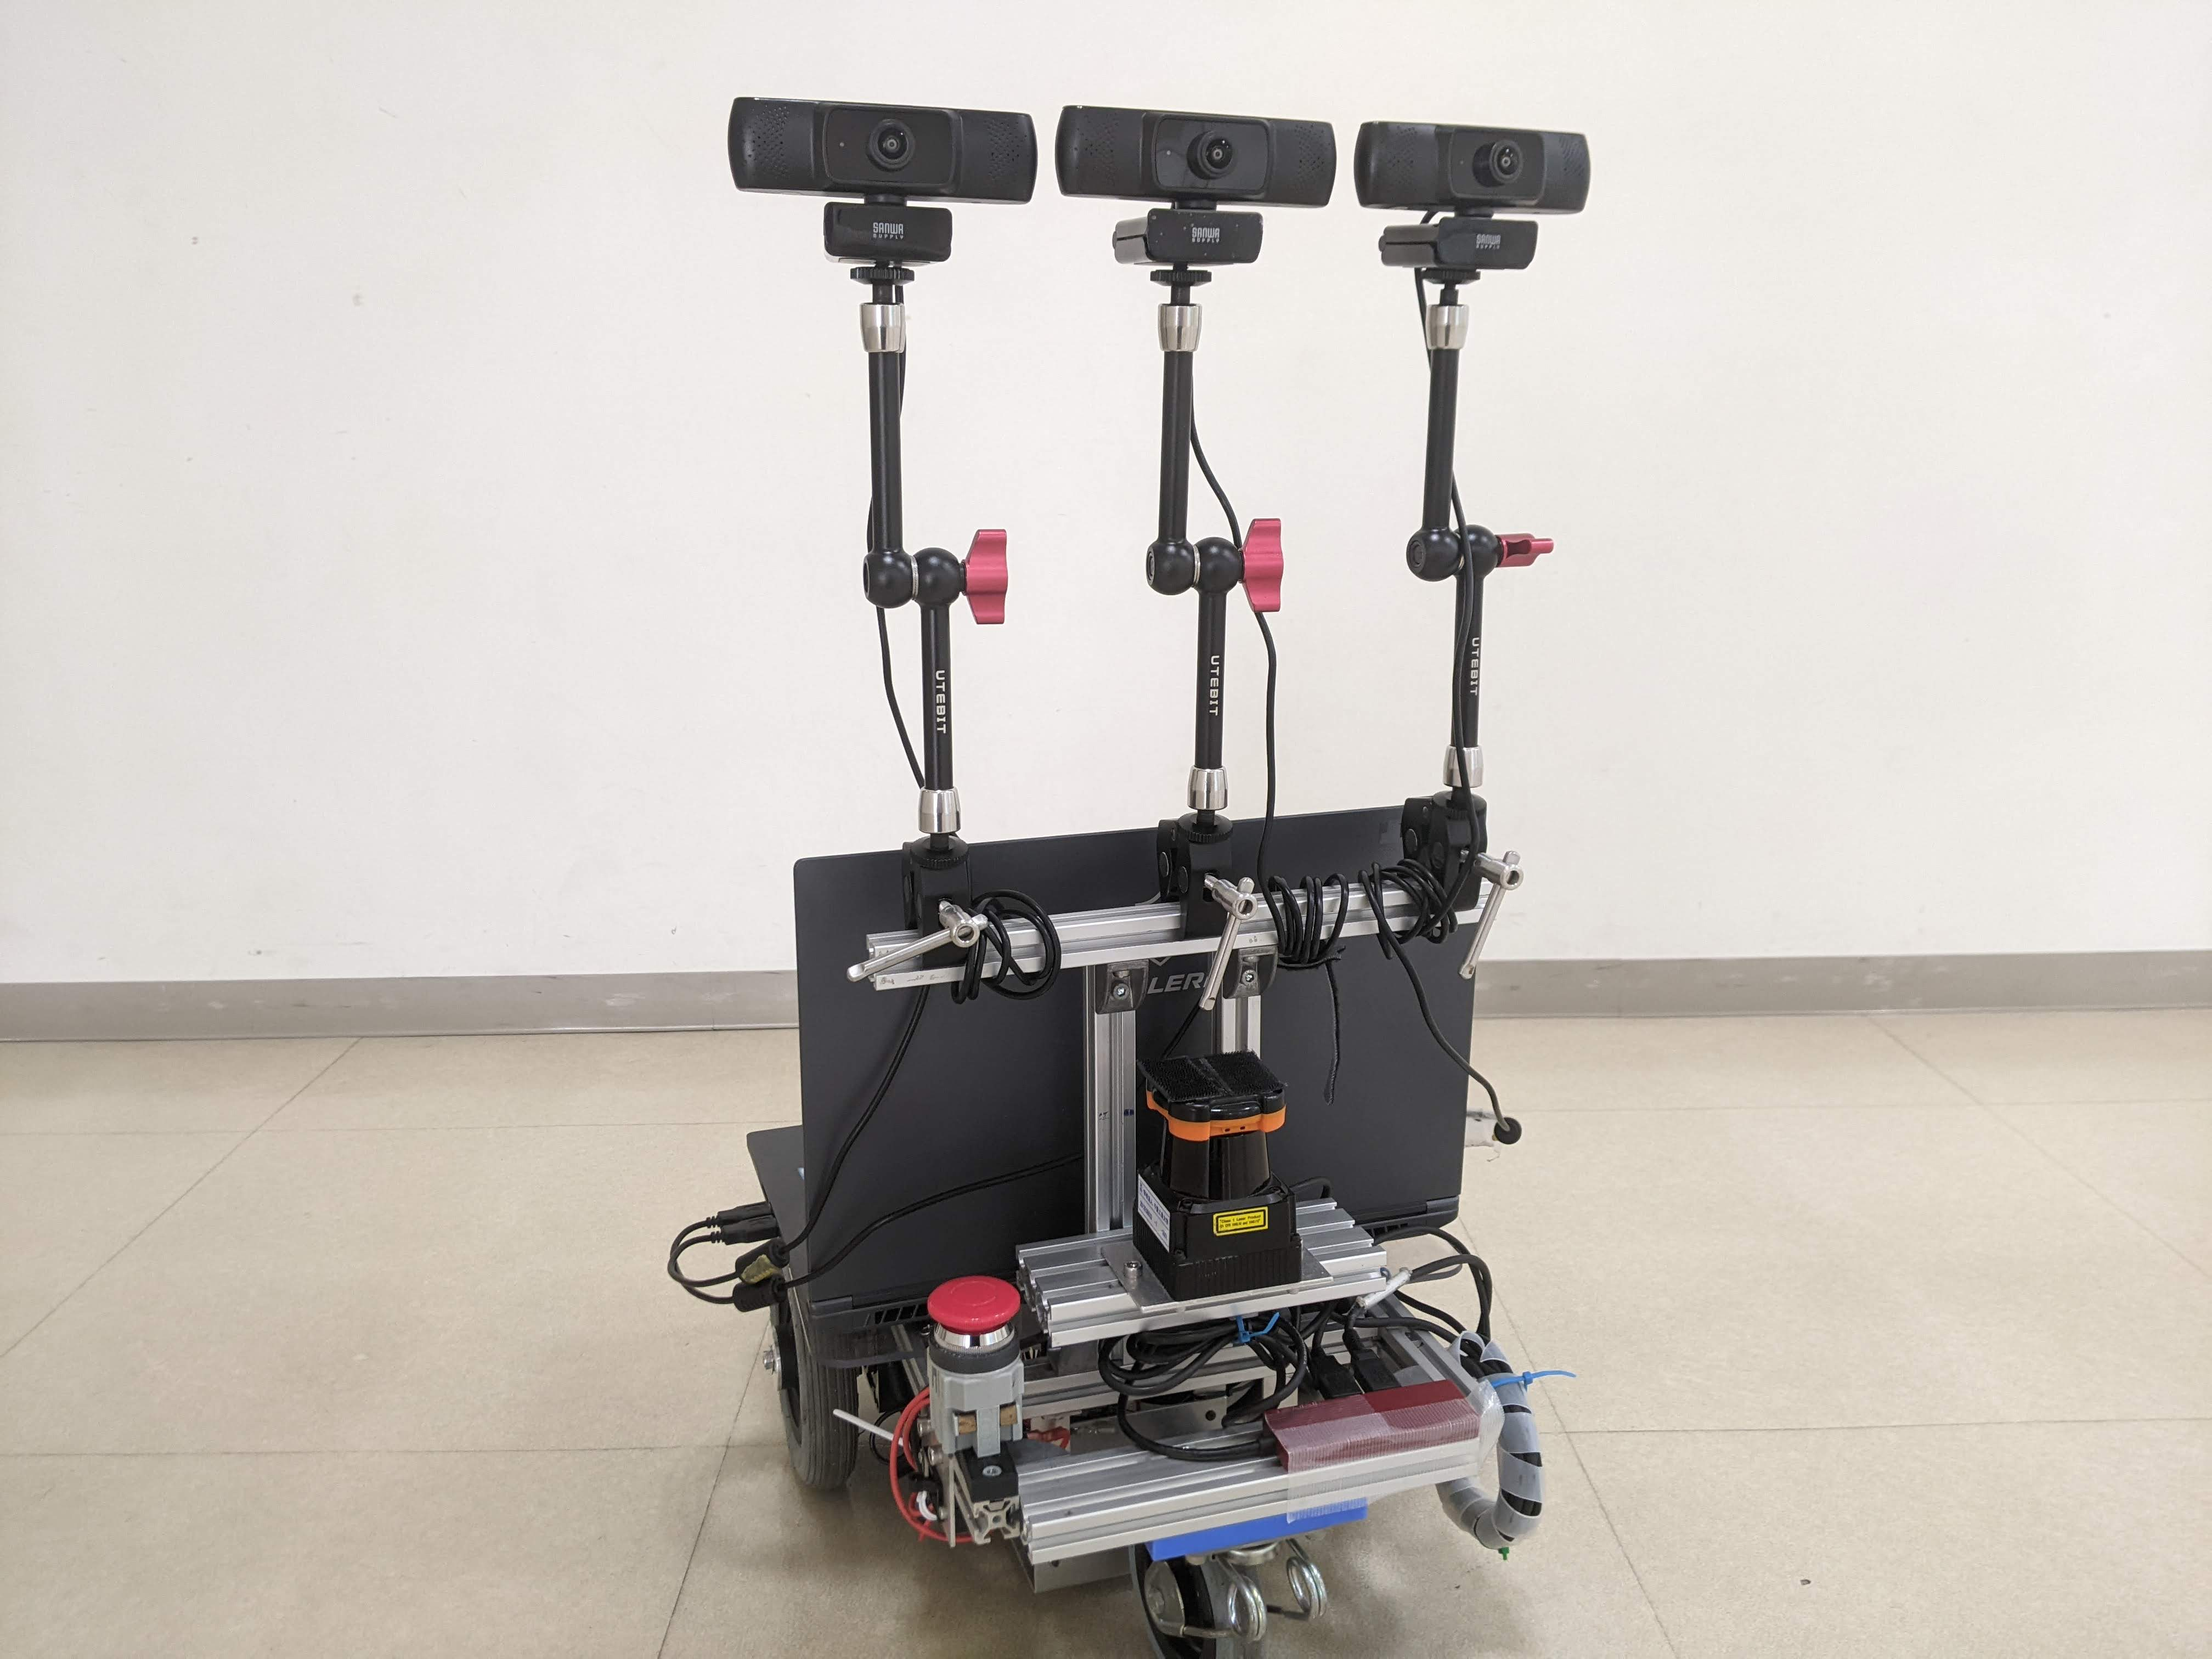
\includegraphics[width=60mm,height=50mm]{./figs/gamma.jpg}
    \caption{orne gamma}
    \end{center}
\end{figure}

\subsection{実験方法}
実験環境には〜でしめした千葉工業大学津田沼キャンパス2号館3階を
用いた.
\begin{figure}[htbp]
    \begin{center}
    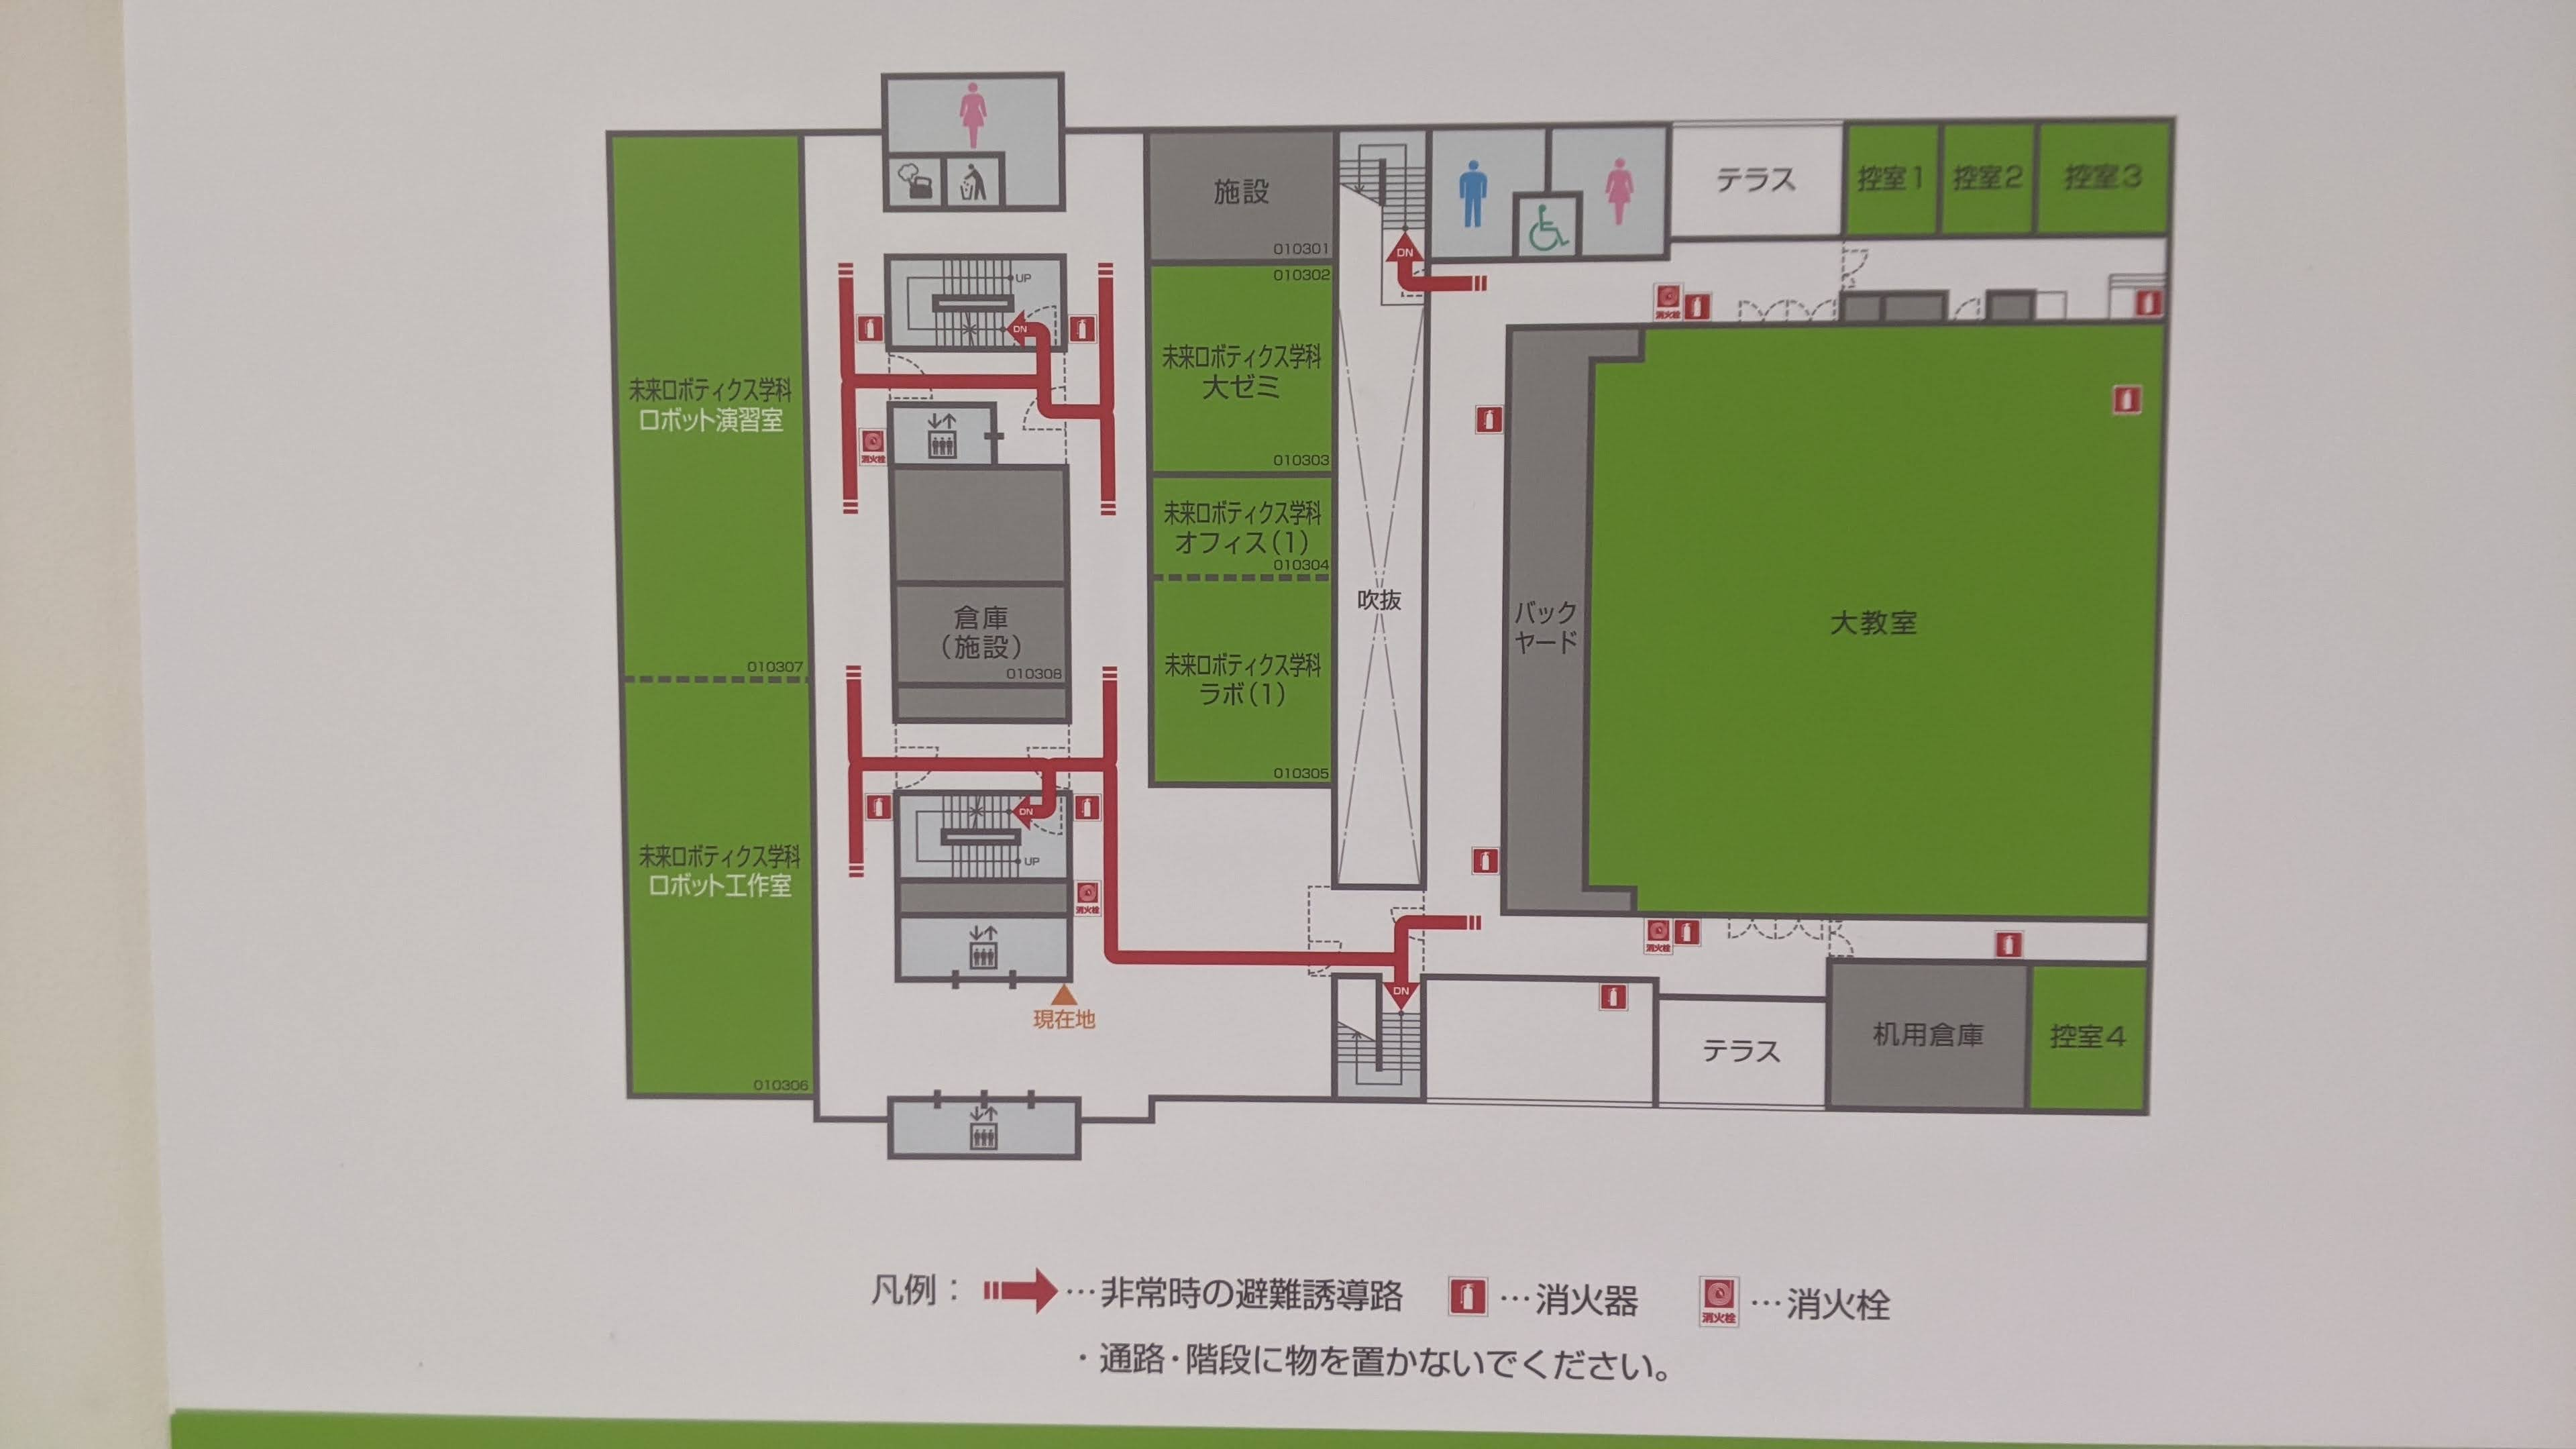
\includegraphics[width=75mm,height=50mm]{./figs/cit3f.jpg}
    \caption{cit3f}
    \end{center}
\end{figure}
まず初めに学習器,通路分類器の訓練を行う.
〜に示した経路を一周し,データを収集する.
模倣学習はオンラインで走行しながら学習を行う.
通路分類器は収集したデータを用いて,30epoch学習を行う.
実験で用いるシナリオについては島田らが用いた50例のシナリオの中から
図中に示したエリアの7例を抽出した.
その際,~のように1.地図ベースの制御器で通行が困難な場所が含まれるもの.
〜のように2.その場で「右を向く」といった学習器の出力を用いた走行では達成が困難なもの
を除外している.
出発地までは人がジョイスティックにより
ロボットを操作し,初期位置でのロボットの向きもシナリオに基づいてセットした.
〜に実験に用いたシナリオ例を示す.
\begin{figure}[htbp]
    \begin{center}
    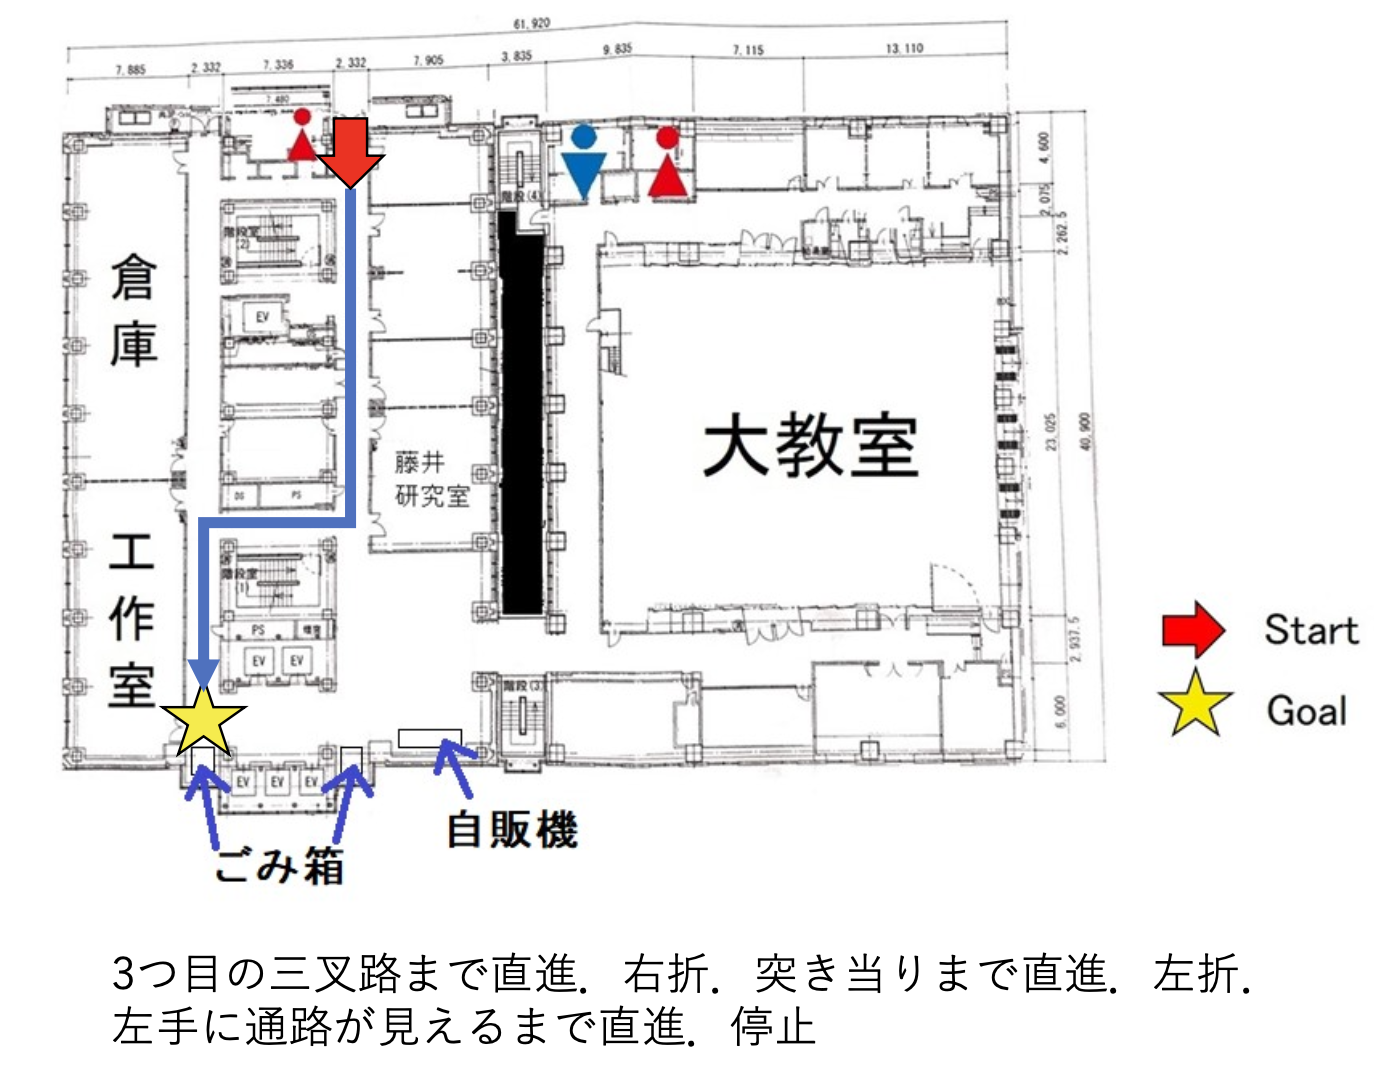
\includegraphics[width=75mm,height=50mm]{./figs/scenario24.png}
    \caption{scenario24}
    \end{center}
\end{figure}
\subsection{実験結果}
結果として,抽出した7例のうち,7例で人間の介入なしで,
指定された経路に沿って走行し目的地へと到達した.
この7例では,模倣学習側,及び通路検出の双方で人間の介入なしで目的地へ到達.

% \begin{table}[h]
%  \caption{Type size and typefaces for papers}
%  \label{tbl: table1}
%  \centering
%  \footnotesize
%  \begin{tabular}{|p{7zw}|c|c|c|}
%   \hline 
% 	適用場所	&日本語	&欧文 \\\hline
% 	標準のフォント	&明朝体 9pt	&Times New Roman 9pt \\\hline
% 	日本語表題	&ゴシック体 14pt	&Arial 14pt \\\hline
% 	日本語副表題	&ゴシック体 12pt	&Arial 12pt \\\hline
% 	英語表題	&-&Times New Roman 12pt \\\hline
% 	英語副表題	&-&Times New Roman 10pt \\\hline
% 	日本語著者名	&明朝体 10pt &-\\\hline
% 	英語著者名	&-&Times New Roman 9pt \\\hline
% 	アブストラクト・キーワード	&-&Times New Roman 9pt \\\hline
% 	大見出し	&ゴシック体 10pt	&Arial 10pt \\\hline
% 	中見出し	&ゴシック体 9pt	&Arial 9pt \\\hline
% 	図・表の番号・タイトル	 &-&Times New Roman 9pt \\\hline
% 	文献	&明朝体 8pt	&Times New Roman 8pt \\
%   \hline
%  \end{tabular}
% \end{table}
\section{結言}
本稿では,条件付き模倣学習によって訓練した学習器を用いた走行に対して,
目標方向の生成を目的として,トポロジカルなナビゲーション追加を行った.
カメラ画像のみに基づいて,目的地へのナビゲーションが可能であることを
実験により確認した.
今後は実験環境を屋外などのより広い環境へと拡張する予定である.

本稿はあくまでも予稿原稿を作成するためのガイドラインを示したものです.改行幅やフォントの設定などについては,原稿の内容や量に合わせて適宜判断していただき,原稿を作成してください.
また,本稿はSICE-SIの予稿原稿の書き方\cite{SI}\cite{SIbook}\cite{WebPage}を参考に,\TeX 用書式を用意したものです.適宜sice-si.clsを変更して使用してください.


% %参考文献
% % \begin{thebibliography}{99}
% %     \bibitem{SI}
% %     計測太郎,制御花子:
% %     ``SICE SI予稿原稿の書き方(サンプル)'',
% %     {\it 計測自動制御学会SI部門講演会SICE-SI予稿集},
% %     pp.0000--0000 (20??)
% % \end{thebibliography}

\printbibliography[title=参考文献]

\end{document}
